\chapter{Experimental Setup}

\section{Relativistic Heavy Ion Collider}
The Relativistic Heavy Ion Collider (RHIC) at Brookhaven National Laboratory (BNL), shown in Fig.~\ref{rhic_config}, is a versatile high energy collider~\cite{RHIC_Overview}. Since year 2000, RHIC has successfully collided $p$ + $p$, $p$ + Al, $p$ + Au, $d$ + Au, $^3$He + Au, Cu + Cu, Cu + Au, Au + Au, and U + U at different energies. The top  energy for the gold ions is 100 GeV/$u$ and that for protons is 250 GeV. A major scientific goal of  RHIC is to study the properties of hot, dense and strongly interacting quantum chromodynamics (QCD) matter created in the laboratory. Meanwhile, as the world-only polarized proton high energy collider, RHIC allows the experimental studies of nucleon's spin structure. Reviews of recent achievements and future of the RHIC spin program can be found in~\cite{RHIC_Spin}.

\begin{figure}[htbp]
\centering
\includegraphics[keepaspectratio,width=0.85\textwidth]{rhic_star/RHIC_Configration.pdf}
\figcaption{The RHIC accelerator complex.}
 \label{rhic_config}
\end{figure}

The process of accelerating gold ions are show in Fig.~\ref{rhic_acc}. Negatively charged (Q = -1) gold ions from the pulsed sputter ion source are partially stripped of electrons in Tandem Van de Graaff, and accelerated to the energy of 1 MeV/$u$. The ions are stripped further (Q = +32) at the exit of the Tandem and then delivered to the Booster Synchrotron through a transfer line. The ions are accelerated to 95 MeV/$u$ in the Booster, and stripped again at the exit to achieve a charge state of Q = +77. The ions are then delivered to the Alternating Gradient Synchrotron (AGS) in 24 bunches. In the AGS, the ions beam are de-bunched, re-bunched to four bunches and accelerated to 10.8 GeV/$u$. The gold ions are fully stripped to the charge state of Q = +79 at the exit from the AGS. These four bunches, one bunch at a time, are injected to the RHIC ring through the AGS-to-RHIC beam transfer line. Once in RHIC, the ions are accelerated to 100 GeV/$u$ (typically, other energies are possible). The protons are accelerated in a different process. They are first accelerated to 200 MeV in a linear accelerator (Linac) before being delivered to the Booster, then to the AGS, and finally to RHIC ring.

RHIC consists of two 3.8 km quasi-circular concentric rings on a common horizontal plane, one (``Bule Ring'') for clockwise and the other (``Yellow Ring'') for counter-clockwise. There are six interaction points on RHIC rings, among which are located four experiments, called STAR at 6 o'clock, PHENIX at 8 o'clock, PHOBOS at 10 o'clock and BRAHMS at 2 o'clock. PHOBOS and BRAHMS experiments decommissioned in 2005 and 2006, respectively, after completing their physics goals. While the STAR and PHENIX experiments are still operating as of today.

An upgrade to Electron Ion Collider (EIC) known as eRHIC~\cite{eRHIC}, focused on the structure and interactions of gluon-dominated matter~\cite{EIC_Physics}, is being planed. The new facility will deliver electron-nucleon luminosity of 10$^{33}$-10$^{34}$ cm$^{-2}$sec$^{-1}$ for collisions of 15.9 GeV polarized electrons on either 250 GeV polarized protons or 100 GeV/$u$ heavy ion beams. The facility will also be capable of providing an electron beam energy of 21.2 GeV, at reduced luminosity. 

\begin{figure}[htbp]
\centering
\includegraphics[keepaspectratio,width=0.7\textwidth]{rhic_star/RHIC_AccGold.png}
\figcaption{RHIC acceleration scenario for Au beam~\cite{RHIC_Configuration}.}
 \label{rhic_acc}
\end{figure}

\section{STAR Detector}
\label{stardet}
The Solenoidal Tracker at RHIC (STAR) ~\cite{STARdet}, composed of several sub-detector systems, is a multi-purpose particle detector. The large and uniform acceptance (0$<\phi<$ 2$\pi$, $|\eta|<$ 1) of the STAR detector, makes it well suited for event-by-event characterization of high charged particle multiplicity heavy-ion collisions. Figure~\ref{star} shows the layout of the STAR detector complex. The center of STAR serves as the original point. The $x$ direction is pointing to the south and the $y$ direction is pointing up (away from the earth surface). The $z$ direction is the beam pipe direction with the west direction as being positive. The whole system except the Muon Telescope Detector (MTD) is enclosed in a homogeneous magnetic filed generated by a solenoidal magnet. The magnetic field direction is parallel to the beam pipe and the maximum magnetic field is $|B_{z}|$ = 0.5 T. STAR can be operated in full field, reverse full field and half field magnetic field configurations.

\begin{figure}[htbp]
\centering
\includegraphics[keepaspectratio,width=1\textwidth]{rhic_star/STAR.png}
\figcaption{Perspective view of the STAR detector.}
 \label{star}
\end{figure}

Charged particle tracking close to the interaction region is accomplished by the Heavy Flavor Tracker (HFT)~\cite{HFTdet}. The HFT was completely installed before 2014 physics run, and successfully collected $\sim$1.2 billion minimum-bias Au + Au events in the 2014 run and $\sim$1 billion $p$ + $p$ , $\sim$0.6 billion $p$ + Au events in the 2015 run. The HFT consists of four cylindrical silicon detector layers and covers $|\eta|<$ 1.2. Two innermost silicon PiXeL detector (PXL) layers are the first application of the state-of-the-art thin Monolithic Active Pixel Sensors (MAPS) technology in a collider environment. The outermost layer is the Silicon Strip Detector while the Intermediate Silicon Tracker (IST) layer sits in the middle of the HFT. The high spatial resolution of the tracker allows us to reconstruct the secondary decay vertices of short-lived particles, such as the D$^{0}$, D$^{+/-}$, D$_{s}$ mesons. A preliminary measurement of the D$^{0}\rightarrow$ K$\pi$ production in Au + Au at $\sqrt{s_{NN}}=$ 200 GeV using 125M minimum-bias data collected in year 2014 is shown in Fig.~\ref{D0signal}~\cite{D0plot}. The combinatorial background is suppressed by $\sim$4 orders of magnitude achieved by the HFT. 

\begin{figure}[htbp]
\centering
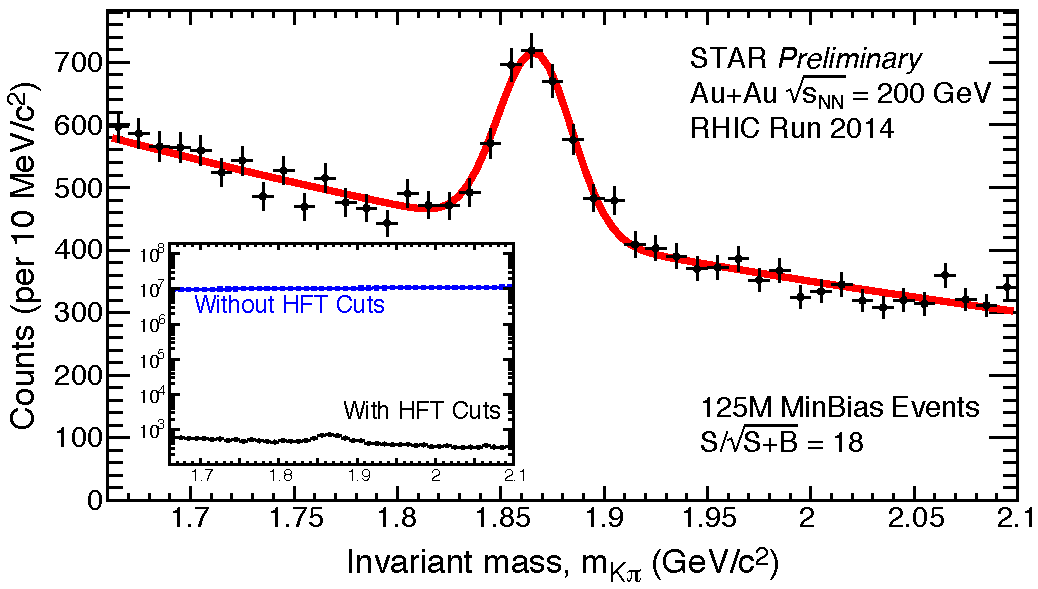
\includegraphics[keepaspectratio,width=0.8\textwidth]{rhic_star/D0_Signal.pdf}
\figcaption{D$^{0}\rightarrow$ K$\pi$ production in Au + Au at $\sqrt{s_{NN}}=$ 200 GeV using 125M  minimum-bias data collected in year 2014~\cite{D0plot}. The insert plot shows the suppression of combinatorial background by $\sim$4 orders of magnitude achieved by the HFT.}
 \label{D0signal}
\end{figure}

The Time Projection Chamber (TPC)~\cite{TPCdet} is the main tracking device in STAR, whose inner and outer field cages are located at radial distance of 50 and 200 cm respectively from the beam axis. The TPC is 4.2 meters long and it covers a pseudo-rapidity range $|\eta|<$ 1.8 and full azimuthal. The TPC provides charged particle tracking, momentum and ionization energy loss ($dE/dx$) measurements for particle identification. The TPC is surrounded by the Time-of-Flight (TOF)~\cite{TOFdet} detector which covers $|\eta|<$ 0.9 and complete azimuthal symmetry. The TOF measures the charged particle velocity and enable us to reject the slow hadron from electrons, opening an opportunity for dielectron analysis at STAR. Following the TOF is the Barrel ElectroMagnetic Calorimeter (BEMC)~\cite{BEMCdet}. The BEMC (0$<\phi<$2$\pi$, $|\eta|<$ 1) is used to trigger on and measure high transverse momentum electrons, photons. In addition, the BEMC also provides prompt charged particle signals essential to discriminate against pileup tracks in the TPC in high luminosity $p$ + $p$ collisions. Outside of the BEMC is the STAR magnet system. The magnetic coils and steels can reject most hadrons while the cross-section of muon in the magnet is small. The muons can penetrate the coils and steels and reach the MTD~\cite{MTDdet}, which is located at the outermost of STAR. The MTD system was fully installed in early 2014 and it covers about 45\% in azimuthal within $|\eta|<$ 0.5. The MTD can trigger on and identify muons based on its precise timing and modest position resolution.

Along the beam axis, there are three fast trigger detectors: Beam Beam Counter (BBC)~\cite{BBCdet}, Vertex Position Detector (VPD)~\cite{VPDdet}, Zero Degree Calorimeter (ZDC)~\cite{ZDCdet}.  The BBC consists of two collections of four scintillator annuli centered around the beam pipe, each located 3.74 m from the interaction region. The two inner (18 channels) and two outer (18 channels) annuli together cover a pseudo-rapidity range of ~2.1 $<|\eta|<$ 5.0, and there is a slight overlap between the inner and outer annuli. The BBC acts as a main detector in the $p$ + $p$ minimum-bias trigger. The minimum-bias trigger requires at least one hit in the two inner annuli of each side coincidentally. This trigger corresponds to a $p$ + $p$ cross section of  $\sim$26.1 $\pm$ 0.2 (stat.) $\pm$ 1.8 (sys.) mb, 87$\pm$8\% of the total none singly diffractive cross section. The VPD consists of two assemblies, and each assembly is composed of 19 channels (units) while only 16 channels are used for STAR trigger input. The two assemblies of the VPD are symmetrically located at a distance of 5.7 m with respect to the interaction region and the VPD covers a pseudo-rapidity of 4.24 $<|\eta|<$ 5.1. The VPD is fully integrated into the STAR trigger system and provides the primary input to the minimum-bias trigger in nucleus-nucleus collisons. The precise timing information from the VPD detector channels is used both in online ($\sim$150 ps in $\sqrt{s_{NN}}$ = 200 GeV Au + Au) and offline ($\sim$30 ps in $\sqrt{s_{NN}}$ = 200 GeV Au + Au) to measure the $z$ position of primary vertex and provide ``start time'' for the TOF and MTD. The two assemblies of ZDC are directly in line with the STAR beam pipe, located 18 m from the interaction point. The ZDC is used for measuring the energy in neutral particles surviving the heavy-ion collisons. The more overlap of ions, the less neutral particles survive from the collisions, and the smaller signal in the ZDC. This makes the ZDC sensitive to the centrality of the collisions. Each experiment at RHIC has a complement of ZDCs for triggering, monitoring luminosity, and cross-calibrating the centrality triggering between experiments.

In the next few sections, we will focus on the TPC and TOF which play a direct role in this dielectron analysis.

\subsection{Time Projection Chamber}
\label{detector:TPC}

The Time Projection Chamber (TPC) is the central element of STAR, and it records the charged particle tracks, momenta and ionization energy loss for particle identification. At the time it was built, the STAR TPC was the largest TPC in the world with a 4.2 m long and 4 m in diameter.  It sits in the STAR solenoidal magnet which produces a maximum 0.5 T magnetic field,  allowing for the momenta measurement.

Figure~\ref{tpccage} shows the schematic view of the STAR TPC. The TPC is an empty volume of P10 (90\% Ar + 10\%CH$_{4}$) gas regulated at 2 mbar above atmospheric pressure in a uniform electric field of $\sim$135 V/cm which is along z direction and defined by a thin conductive Central Membrane (CM, held at -28 kV) at the center of  the TPC, concentric field-cage cylinders and the readout end caps (held at ground potential). The P10 gas has long been used in TPCs with advantage of a fast drift velocity peaking at a low electric field. Operating on the peak of the velocity curve makes the drift velocity stable and insensitive to the small variations in temperature and pressure. The transverse diffusion and longitudinal diffusion at 0.5 T are about $\sigma_{T}$ = 3.3 mm (230 $\mu$m/$\sqrt{cm}$) and $\sigma_{L}$ = 5.2 mm (360 $\mu$m/$\sqrt{cm}$), respectively, after drifting the full length of TPC. The longitudinal diffusion width sets the scale for the resolution of the tracking system in the drift direction.

\begin{figure}[htbp]
\centering
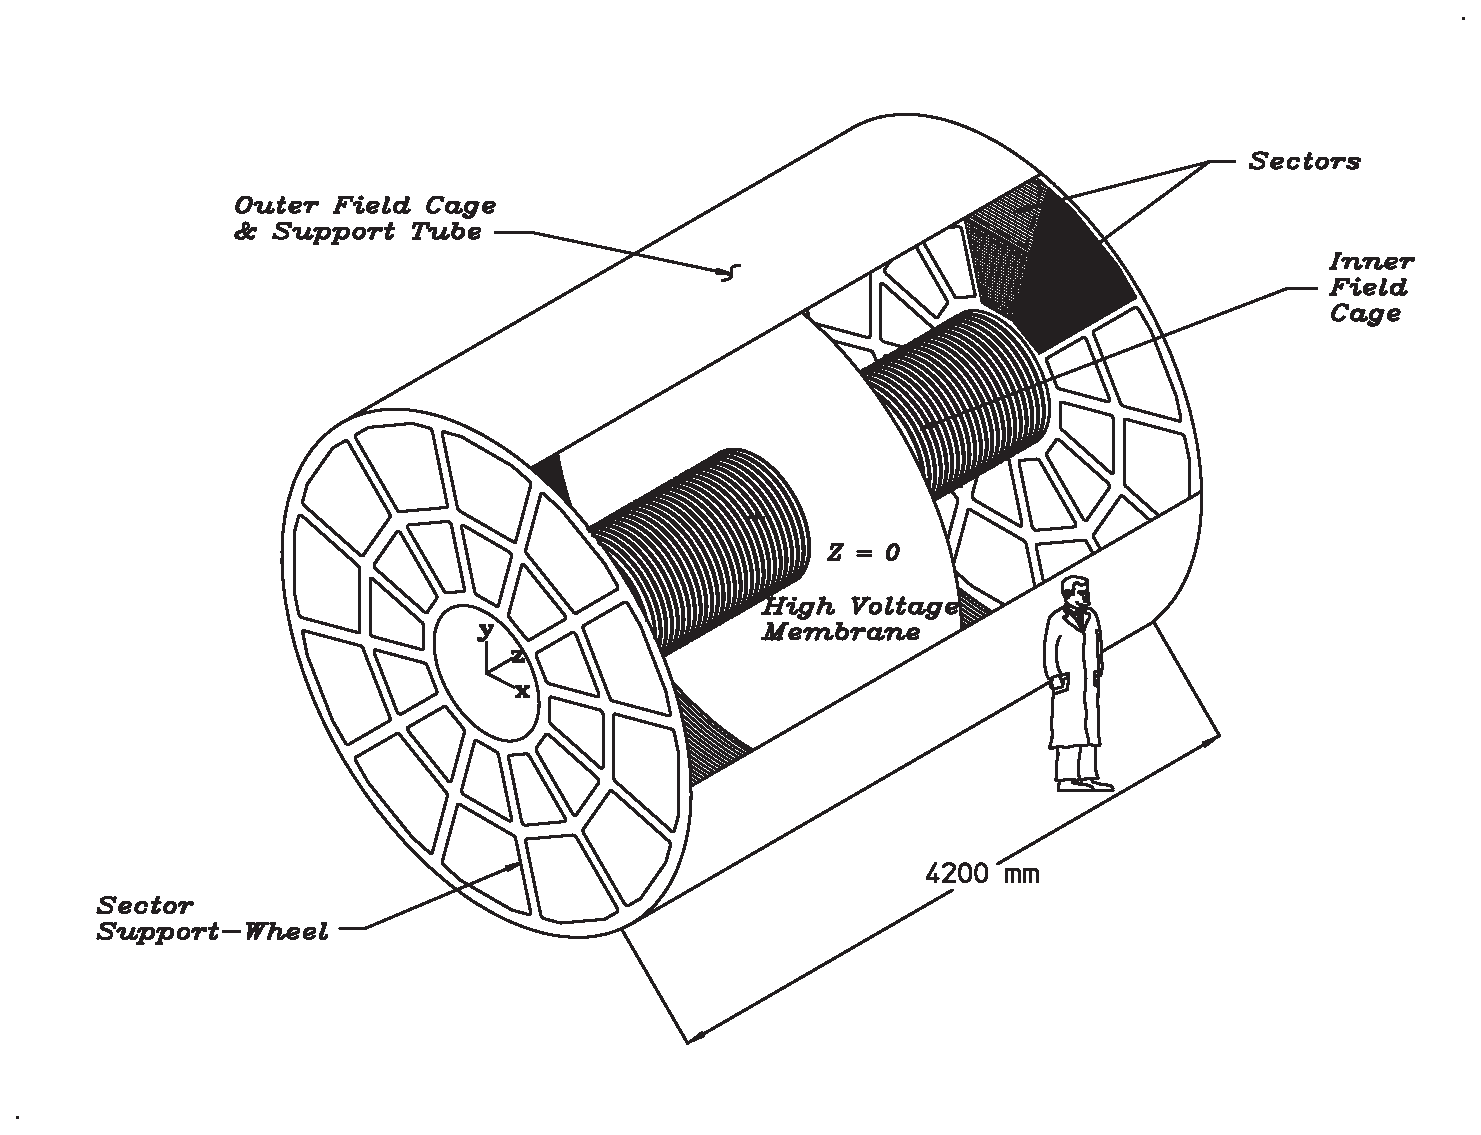
\includegraphics[keepaspectratio,width=0.9\textwidth]{rhic_star/tpcman.eps}
\figcaption{The schematics of the STAR TPC.}
 \label{tpccage}
\end{figure}

There are 12 sectors with 45 pad rows, arranged as on a clock face, in each readout end cap. Each sector is then divided into an outer and inner sub-sector as shown in Fig.~\ref{padplane}. The outer sub-sector has a continuous pad coverage to optimize the $dE/dx$ resolution and tracking resolution. The inner sub-sector with smaller pads, located at the region of highest track density, is optimized for good two-hit resolution. The use of separate pad rows instead of continuous pad coverage for inner sub-sector is due to the constraint imposed by the available packing density of the front end electronics channels on that time.

\begin{figure}[htbp]
\centering
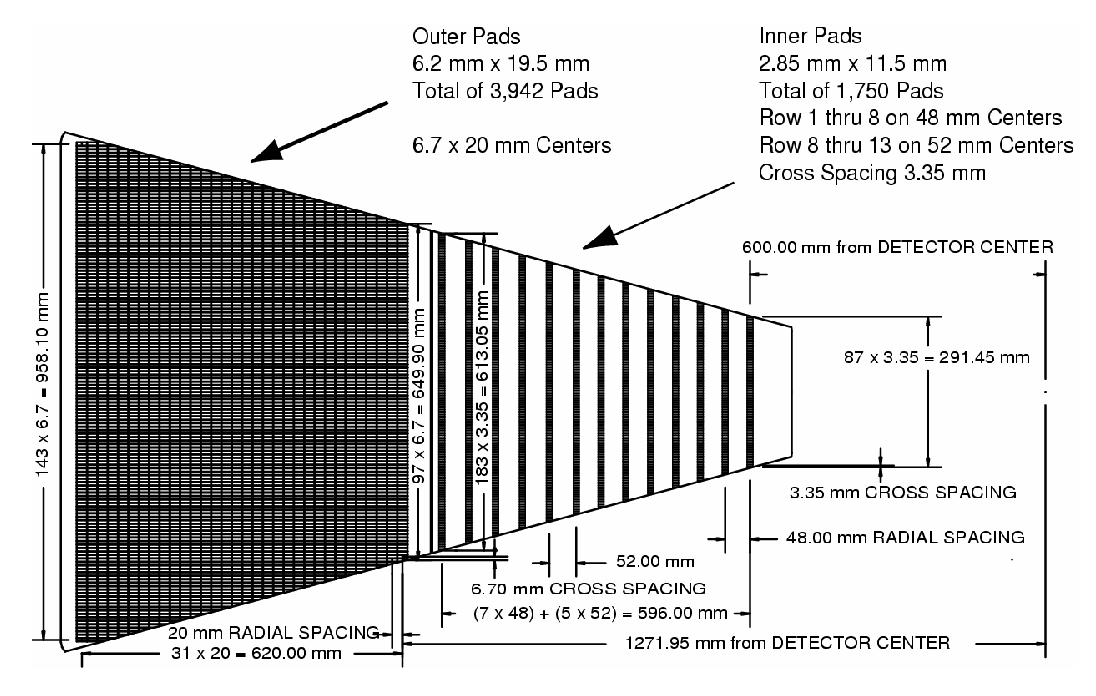
\includegraphics[keepaspectratio,width=0.8\textwidth]{rhic_star/padplane.eps}
\figcaption{ The anode pad plane with one full sector shown. The inner subsector is on the right and it has small pads arranged in widely spaced rows. The outer subsector is on the left and it is densely packed with larger pads.}
 \label{padplane}
\end{figure}

\begin{figure}[htbp]
\centering
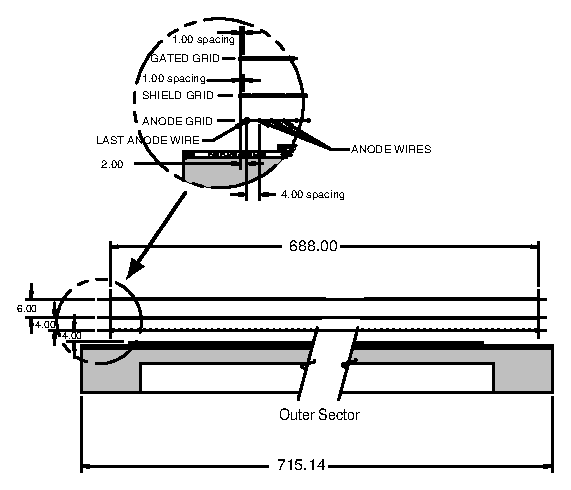
\includegraphics[keepaspectratio,width=0.8\textwidth]{rhic_star/outer_wires.eps}
\figcaption{ A cut-away view of an outer sub-sector pad plane. The cut is taken along a radial line from the center of the TPC to the outer field cage so the center of the detector is to the right. The figure shows the spacing of the anode wires relative to the pad plane, the ground shield grid, and the gated grid. The bubble diagram shows additional detail about the wire spacing. The inner subsector pad plane has the same layout except the spacing around the anode plane is 2 mm instead of the 4 mm shown here. All dimensions are in millimeters.}
 \label{mwpc}
\end{figure}

As charged particles pass through the TPC volume, they ionize the working gas along their path, releasing electrons and positive ions. The electrons drift toward the end cap and are collected by the Multi-Wire Proportional Chambers (MWPC). The MWPC is composed of a pad plane and three wire planes: a gating grid, a ground pane, and anode wires, shown in Fig.~\ref{mwpc}. The gating grid is ``close'' when the wires are alternately biased $\pm$75 V. Thus it blocks the entry of electron from TPC volume into MWPC and positive ions produced in MWPC into TPC volume. The gating grid is ``open'', biasing the wires to the same potential (typically -110 V), when recording the collision event. The positive ions are too slow to escape during the open period and get captured during the closed period. Once the electrons enter the MWPC, much more electrons are produced through avalanche in the high field inducing a signal on the readout plane. These induced signals  are used for tracing the position of ionization clusters along the charged particle tracks. The clusters are found separately in the $x$-$y$ plane ($r$-$\phi$ plane) and in z direction. The $x$ and $y$ coordinates of a cluster are determined by the charge measured on adjacent pads in a single pad row while the $z$ coordinate is determined by measuring the drift time of a cluster from the original point to the anodes on the endcap multiplying the average drift velocity (typically $\sim$5.45 cm/$\mu$s, but calibrated every few hours to account for atmospheric pressure variations by using artificial tracks created by lasers beams~\cite{TPClaser}). The particle tracks are then reconstructed from the individual clusters (hits) found in the TPC and the reconstruction is achieved with a Kalman filter routine. The resulted track collection from the TPC is combined with any other available tracking detector reconstruction hits and then refit. The reconstructed tracks are called global tracks. The primary interaction vertex is fit from the global tracks with at least ten hits. The Distance of Closest Approach (dca) to the fit primary vertex is calculated for each global track. Iterations are made such that global tracks with dca $>$ 3 cm are excluded from subsequent primary vertex fitting. The vertex resolution is inversely proportional to the square root of the number of tracks used in the calculation and can reach 350 $\mu$m when there are more than 1000 tracks. The tracks (global tracks with dca $<$ 3 cm) originated from the primary vertex are refit including the primary vertex to improve the momentum resolution, so called primary tracks. The momentum resolution of primary track in $p$ + $p$ collisions is approximately $\delta p_{T}/p_{T} \approx$ 1\% + 0.5\% $\times$ $p_{T}$.

Particle identification can be realized in the TPC through the $dE/dx$. The mean rate of $dE/dx$ of a charged particle passing trough the TPC can be described by the Bichsel function~\cite{Bichsel}. Different particle species with the same momentum may result in different $dE/dx$. The $dE/dx$ is extracted from the energy loss measured on up to 45 padrows. However, the mean $dE/dx$ is impossible to be accurately measured due to the ionization fluctuations and finite track length over the energy loss measured. Therefore, the most probable energy loss is measured by truncating the largest 30\% ionizations clusters. The typical resolution of $dE/dx$ in Au + Au collisions is $\sim$8\%, which makes the $\pi/K$ separation up to p $\sim$0.7 GeV/$c$ and ($\pi,K)/p$ separation up to p $\sim$1.1 GeV/$c$.

\subsection{Time of Flight}

The full barrel Time-of-Flight (TOF), based on the Multi-gap Resistive Plate Chamber (MRPC)~\cite{STARTOFmrpc0}, was completely installed in year 2010. The MRPC technology was first developed by the ALICE group~\cite{ALICETOFmrpc} to provide a cost-effective solution for large area Time-of-Flight coverage. The barrel TOF, covering $|\eta|<$ 0.9 and 2$\pi$ azimuthal, is composed of 120 trays, with 60 on east side and 60 on west side. Each tray consists of 32 single-end readout MRPC modules, whose structure is shown in Fig.~\ref{tofmrpc}. The MRPC module consists a stack of floating resistive plates with a series of uniform gas gaps (220 $\mu$m) defined by a nylon monofilament fishing line. The active size of the MRPC module is 61 $\times$ 200 mm$^{2}$. The module has 6 readout pads while each pad has an area of 63 $\times$ 31.5 mm$^{2}$. The interval between two pads is 3 mm wide. The first beam test for the MRPC module at CERN PS-T10 test beam facility using 7 GeV/$c$ pion beam resulted in 65 ps time resolution with greater than 95\% detection efficiency and capability of working at high event rate 500 Hz/cm$^{2}$ ~\cite{STARTOFmrpc0, STARTOFmrpc1}.


\begin{figure}[htbp]
\centering
\includegraphics[keepaspectratio,width=0.8\textwidth]{rhic_star/TOFmrpc.png}
\figcaption{Two side views of MRPC~\cite{TOFdet}. The upper is for long side view and the lower is for short side view.}
 \label{tofmrpc}
\end{figure}

The whole TOF system consists of two parts, the barrel TOF and the VPD. The VPD has been explained in the former section. The VPD provided the ``start'' time of the charged particles while the barrel TOF provides the ``stop'' time. With HPTDC Integral Non-Linearity (INL) correction, T$_{0}$ correction (eliminating relative offsets caused by cable length and electronics), slewing correction (eliminating the time difference caused by different signal amplitude) applied (see details in~\cite{VPDdet,VPDTOFcalib0, VPDTOFcalib1}), the time resolutions of the VPD and barrel TOF can achieve $\sim$30 ps and $<$80 ps in heavy-ion collisions, respectively. With such time resolution, the TOF system significantly improves the particle identification capability. The $\pi/K$ separation momentum range is extended from $\sim$0.7 GeV/$c$ to $\sim$1.6 GeV/$c$ and $(\pi,K)/p$ separation from $\sim$1.1 GeV/$c$ to $\sim$3 GeV/$c$~\cite{tofpid}. Figure~\ref{tofbeta} shows the 1/$\beta$ distribution of different particle species measured by the TOF in U + U at $\sqrt{s_{NN}}$ = 193 GeV. For electron identification, the TOF is used to reject slow hadrons in cross-over $dE/dx$ regions which will be discussed in detail in Chapter~\ref{chap:analysis}. 

\begin{figure}[htbp]
\centering
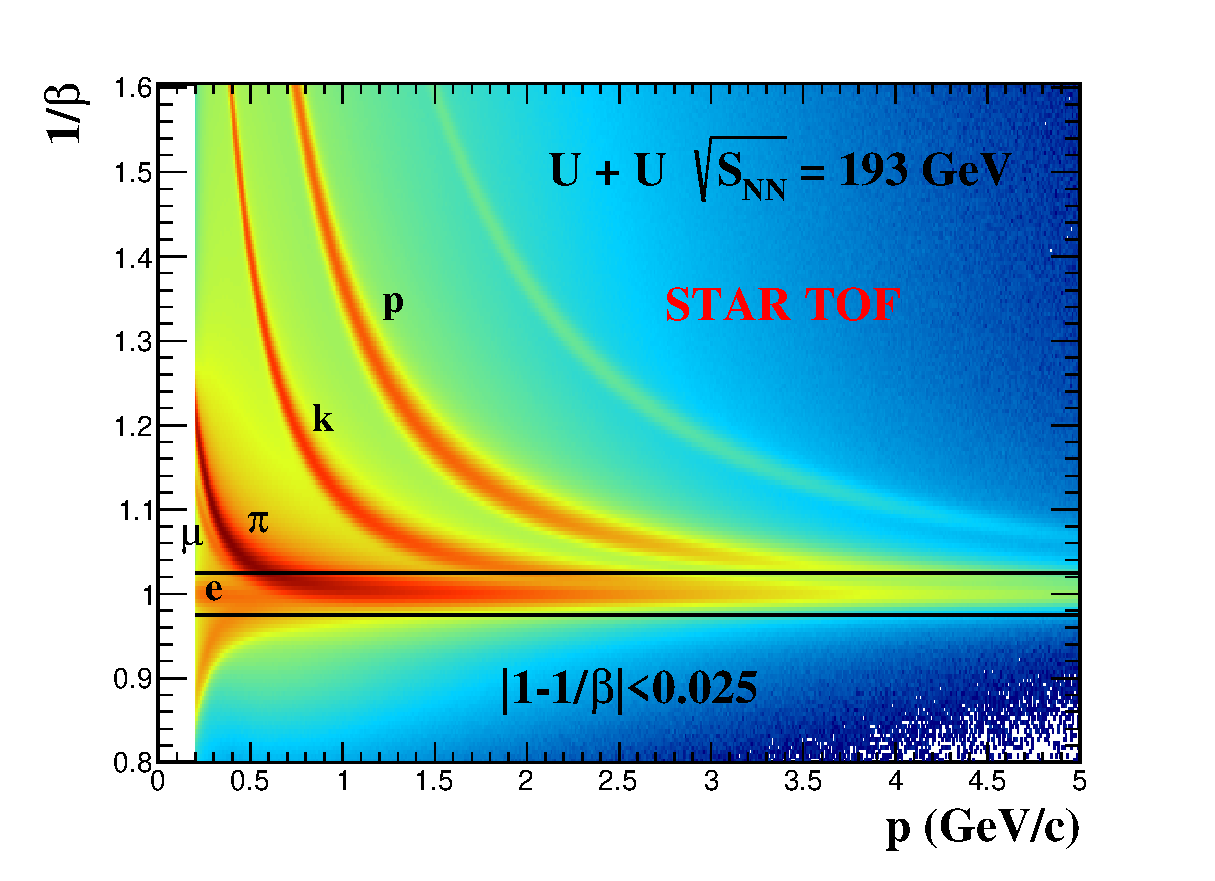
\includegraphics[keepaspectratio,width=0.8\textwidth]{rhic_star/betavsp.eps}
\figcaption{1/$\beta$ distribution for different particle species in U + U collisions at $\sqrt{s_{NN}}$ = 193 GeV.}
 \label{tofbeta}
\end{figure}

%封面是按照制本厂的要求制作的,其中行宽和行高都是固定的,中文标题最多占两行,英文标题最多占三行。如果您的题目超过了这个限制,请缩减题目长度,不要擅自修改模板中的相关配置参数。

